\documentclass{standalone}
\usepackage{tikz}

\begin{document}

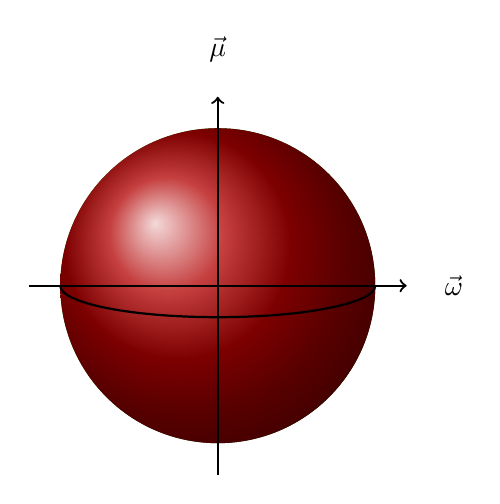
\begin{tikzpicture}[scale=2]
    % Draw the sphere
    \shade[ball color=green!70!black] (0,0) circle (1);
    \shade[ball color=red!70!black] (0,0) circle (1);

    % Draw the axis of rotation
    \draw[->, thick] (-1.2,0) -- (1.2,0);
    \draw[->, thick] (0,-1.2) -- (0,1.2);

    % Label the axis of rotation
    \node at (1.5,0) {$\vec{\omega}$};
    \node at (0,1.5) {$\vec{\mu}$};

    % Draw the equator
    \draw[thick] (-1,0) arc (180:360:1 and 0.2);
\end{tikzpicture}

\end{document}